\newif\ifpdf
\ifx\pdfoutput\undefined
        \pdffalse % pdfLaTeX не используется
\else
        \pdfoutput=1 % используется PDFLaTeX
        \pdftrue
\fi

\documentclass[serif,mathserif]{beamer}
\usepackage{amsmath, amsfonts, epsfig, xspace}
\usepackage{algorithm,algorithmic}
\usepackage{pstricks,pst-node}
\usepackage{multimedia}
\usepackage[normal,tight,center]{subfigure}
\usepackage[utf8]{inputenc}
\usepackage[russian]{babel}
\usepackage[cp1251]{inputenc} % CP1251 или другая кодировка, с UTF8 не дружит bibTeX
\setlength{\subfigcapskip}{-.5em}
\usepackage{beamerthemesplit}
\usetheme{lankton-keynote}



\author[Московченко А. Абрамов Н. Пантелеев И.]{Московченко Анастасия \quad Абрамов Николай\\Пантелеев Игорь }

\title[Отчет\hspace{2em}\insertframenumber/\inserttotalframenumber]{Отчет по второму заданию}

\institute{МГУ им М.В. Ломоносова}

\begin{document}

\maketitle

% \section{Introduction}  % add these to see outline in slides

\begin{frame}
  \frametitle{Цель}
   Проведение разведывательного анализа данных, чтобы опредедлить с каким поставщиком заключить договор
  
\end{frame}

% \section{Main Body} % add these to see outline in slides

\begin{frame}
  \frametitle{Поэтапное описание разведывательного анализа данных}
  Первый этап: 
  
  Рассчитана сумма произведенных мечей в разрезе компании и месяц производства
  Составлена матрица долей сломанных мечей от количества произведенных за каждый месяц использования
\end{frame}   

\begin{frame}
 \frametitle{Поэтапное описание разведывательного анализа данных}
 \begin{figure}[h]
  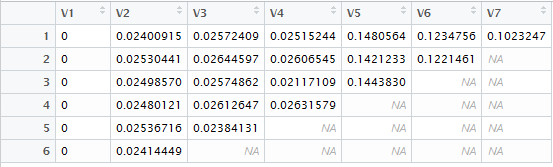
\includegraphics[width=90mm,height=20mm]{table1.png}
   \caption{"harpy.co"}
   \label{Table}
   \end{figure}
   \begin{figure}[h]
   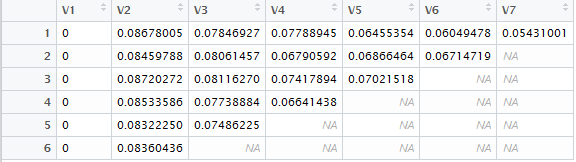
\includegraphics[width=90mm,height=20mm]{table2.png}
   \caption{"westeros.inc"}
   \label{Table}
   \end{figure}
  
\end{frame}

\begin{frame}
  \frametitle{Поэтапное описание разведывательного анализа данных}
  Второй этап:
  
  Усреднив значения матрицы по столбцам, была произведена их запись в вектор нарастающим итогом.
  \begin{figure}[h]
            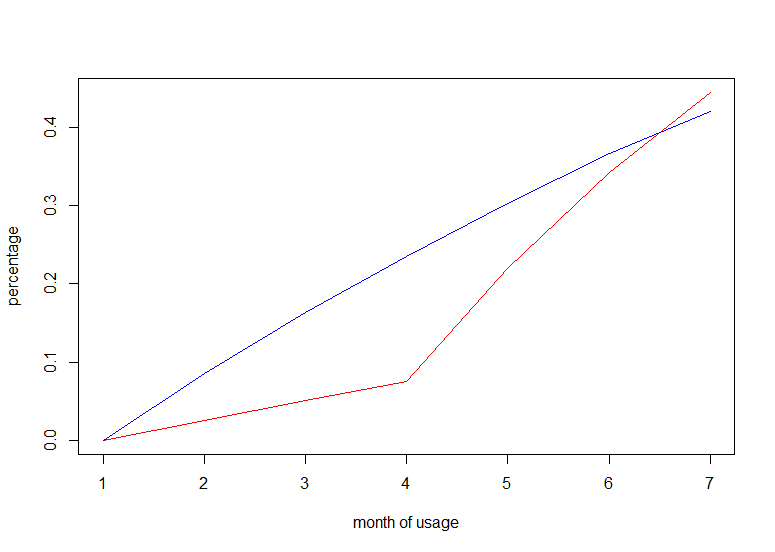
\includegraphics[width=60mm]{Graph1.png}
            \caption{"Красный - harpy.co, синий - westeros.inc"}
            \label{Graph}
  \end{figure} 
\end{frame}




\begin{frame}
 \frametitle{Поэтапное описание разведывательного анализа данных}
  Третий этап:
  Построена линейная регрессия и сделан прогноз на следующие 11 месяцев
  
  \begin{figure}[h]
            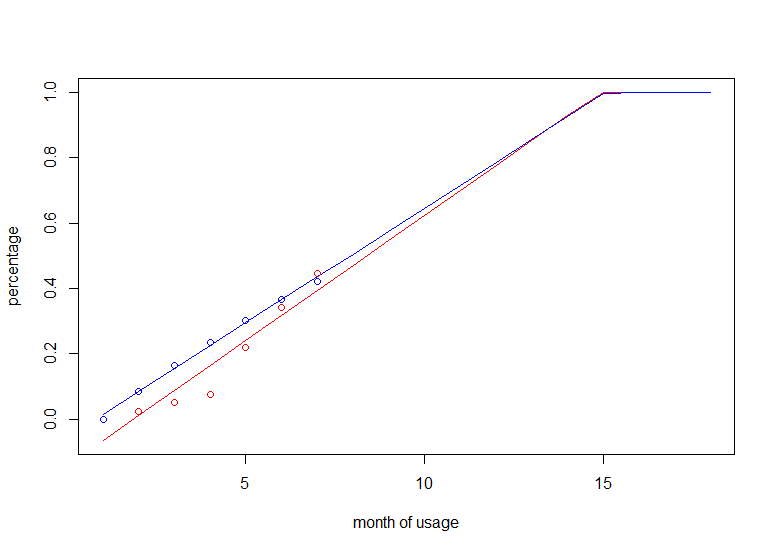
\includegraphics[width=60mm]{Graph2.png}
            \caption{"Красный - harpy.co, синий - westeros.inc"}
            \label{Graph}
      \end{figure}
 
\end{frame}


\begin{frame}
    \frametitle{Поэтапное описание разведывательного анализа данных}
    Четвертый этап:
    Произведен расчет количества целых мечей в разрезе месяц производства.
    Построена диаграмма размаха "Ящик с усами".
      \begin{figure}[h]
            \includegraphics[width=70mm]{pic1.jpg}
            \caption{"Диаграмма размаха Ящик с усами"}
            \label{Graph}
      \end{figure}
     
\end{frame}

\begin{frame}
    \frametitle{Анализ полученных результатов}
    При оценке полученного прогноза можно сделать вывод, что партия мечей у обеих компаний ломается приблизительно в одно и то же время (15 месяцев).
    В начале использования мечи компании "Westeros Inc" ломаются чаще.
    Максимальное и минимальное значения больше у компании "Harpy.co", чем "Westeros Inc". Следовательно компания "Harpy.co" выпускает более крупные размеры партий по сравнению со второй компанией. 
    Медиана колличества целый мечей у компании "Harpy.co" больше, чем у "Westeros Inc". Сдедовательно у компании "Harpy.co" в среднем качество мечей выше.
    После проведенного анализа можно прийти к выводу, что наиболее выгодно заключить контракт с компанией "Harpy.co". 

\end{frame}

\begin{frame}
    \frametitle{Вывод}
    
    \huge{Мы советуем Тириону выбрать "Harpy.co"!}
    
    
    
\end{frame}


\begin{frame}{Задание выполняли}
      \begin{itemize}
            {\small
            \item Московченко Анастасия, студентка 412 группы. Написание презентации, написание кода.
            \item Пантелеев Игорь, студент 411 группы. Написание кода программы и анализ реультатов
            \item Абрамов Николай, студент 412 группы. Написание кода программы и анализ реультатов}
            \end{itemize}
  \end{frame}
\end{document}

